\documentclass[../main.tex]{subfiles}
\begin{document}

Um dieses Problem der Erfassug der Semantik von Code anzugehen, wird der Indexing Prozess für folgende Tests angepasst.

\begin{figure}[ht]
    \centering
    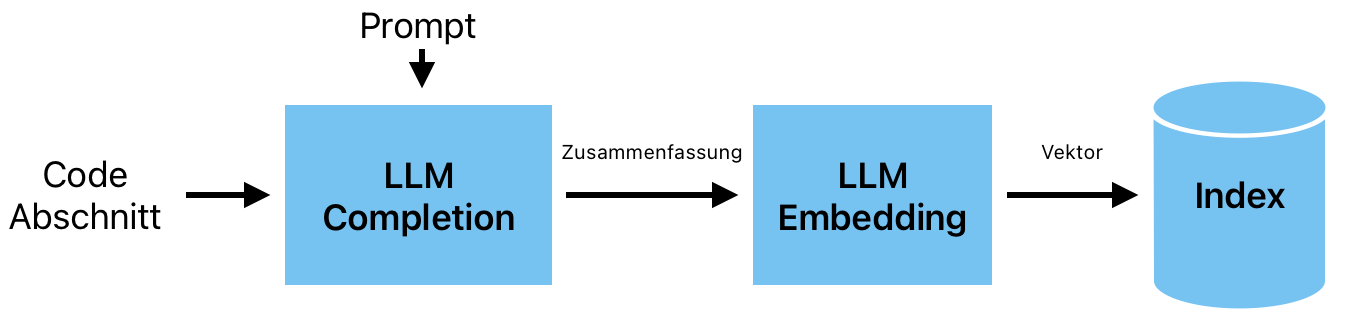
\includegraphics[scale=.6]{"bilder/prozess.png"}
    \caption{Indexing Prozess aus einem Code Abschnitt(Selbst genzeichnet)}
    \label{fig:indexing}
\end{figure}
Dafür wird, wie in Abbildung \ref{fig:indexing} ilustriert, vor der Embedding Generierung ein weiters \gls{LLM} aufgerufen, welches eine Completion durchführt, die als Starttext ein Prompt und den Code Abschnitt erhält.
Das Prompt fordert das \gls{LLM} auf, den erhaltenden Code zusammenzufassem und diese Zusammenfassung wird dann für das Embedding genutzt.
Einerseits kann dem ersten \gls{LLM} durch dieses Prompt mehr Kontext gegeben werden und anderseits ist das Ergebniss dieser ersten Analyse durch das \gls{LLM} ein Text in natürlicher Sprache, der besser von dem Embedding \gls{LLM} erfasst werden kann.
Als Prompt wird folgender Text genutzt:

\begin{lstlisting}
You are a senior software developer. I provide you with a fenced code snippet that is part of a larger codebase.
Do the following things:
1. Summarize what the code does in non technical terms, in 2 sentences.(summary)
2. Briefly describe how the code works. (analysis)
3. Imagine a developer needs to find this code based on its functionality in the codebase. List 3-5 "Where" questions a developer might ask to locate this code, based on its functionality/intent. (questions)
Take your time to do a thorough review and identify meaningful questions.
Return nothing but JSON,
Here is an example:
{
    "summary": "This code snippet sorts an array of numbers. It supports sorting in ascending or descending order.", 
    "analysis": "The code implements the quick sort algorithm to recursively esort an array in ascending  or descending order.",
    "questions": [
        "Where is the code used for sorting data?",
        "Where can I find the array sorting logic?",
        "Where is the code that implements quicksort?"
    ]
}
If the code snippet is empty, just return the text ["NOTHING"].
Do not start with "Here is the JSON object" or similar, just output plain JSON no markdown!


<Code Abschnitt wird hier eingefuegt>
\end{lstlisting}

Im \ref{test3} wird dieses neue Verfahren genutzt und sieben von zehn Fragen können richtig beantwortet werden.
Beim \ref{test4} wird mit dem selben Verfahren das Test Projekt im Zustand aus \ref{test2} untersucht und durch die Verbesserungen werden noch sechs von zehn Fragen richtig beantwortet.
Dabei ist anzumerken, dass die Frage, die beim Vergleich von \ref{test3} und \ref{test4} wegfällt, selbst von einem Menschen nur durch die Dokumentation zu beantworten wäre, da der Codeabschnitt auch für andere Zwecke eingesetzt werden könnte als in der Dokumentation dargelet und durch die Frage gemeint.


\end{document}